%%%%%%%%%%%%%%%%%%%%%%%%%%%%%%%%%%%%%%%%%%%%%%%%%%%%%%%%%%%%%%%%%%%
%
% 4ti2 User Guide
%
% $Id$
%
%%%%%%%%%%%%%%%%%%%%%%%%%%%%%%%%%%%%%%%%%%%%%%%%%%%%%%%%%%%%%%%%%%%

\documentclass[12pt]{article}
\usepackage{amssymb,amsmath,amsthm}
\usepackage{epsfig}


%%%%%%%%%%%%%%%%%%%%%%%%%%%%%%%%%%%%%%%%%%%%%%%%%%%%%%%%%%%%%%%%%%%
\usepackage{verbatim}
%-- Create a verbatim environment which indents itself.
\newenvironment{myverbatim}%
  {\quote\verbatim}%
  {\endverbatim\endquote}

%%%%%%%%%%%%%%%%%%%%%%%%%%%%%%%%%%%%%%%%%%%%%%%%%%%%%%%%%%%%%%%%%%%
%%%%%%%%%%%%%%%%%%%%%%%%%%%%%%%%%%%%%%%%%%%%%%%%%%%%%%%%%%%%%%%%%%%
% To make some comments on the text.
% What is still to do ...
\newcommand{\DefToDo}[2]{%
  \newenvironment{#1}[1]{
    \list{}{\rightmargin0pt}\item\relax\fbox{\rm\textbf{##1 #2:}}\small%
    \marginpar{\footnotesize\fbox{To Do}}
    }{\endlist}}

\DefToDo{ToDo}{ToDo}
\DefToDo{RHX}{Ralf}
\DefToDo{RAMON}{Raymond}
\DefToDo{PETER}{Peter}

%%%%%%%%%%%%%%%%%%%%%%%%%%%%%%%%%%%%%%%%%%%%%%%%%%%%%%%%%%%%%%%%%%%
%%%%%%%%%%%%%%%%%%%%%%%%%%%%%%%%%%%%%%%%%%%%%%%%%%%%%%%%%%%%%%%%%%%

\frenchspacing
\setlength{\parindent}{0pt}
\parskip=1ex plus .25ex minus .25ex
\pagestyle{plain}
\textwidth15cm
\oddsidemargin0.7cm
\textheight20cm

%%%%%%%%%%%%%%%%%%%%%%%%%%%%%%%%%%%%%%%%%%%%%%%%%%%%%%%%%%%%%%%%%%%
\usepackage{url}
%-- Filenames are typeset in this way.
\newcommand\File{\begingroup \urlstyle{sf}\Url}

%-- Command lines are typeset as follows.
\newcommand\Command{\begingroup \urlstyle{sf}\Url}

%-- How sets should appear which automatically adjust the size
%-- of the braces.
\newcommand{\Set}[1]{\left\{#1\right\}}
\newcommand{\setDef}[2]{{#1}\left|\,\vphantom{#1}{#2}\right.}
\newcommand{\SetDef}[2]{\Set{\,\setDef{#1}{#2}\,}}

\newcounter{rhxCounter}
\newenvironment{Steps}%
  {\begin{list}{}{%
   \newcommand{\Step}[1]{\item[##1]\mbox{}}
%  % The number for the top-level item (appears this way in references).
   \renewcommand{\therhxCounter}{\textbf{\arabic{rhxCounter}}}
%  % This is how it appears in the enumeration
   \renewcommand{\makelabel}[1]{\stepcounter{rhxCounter}%
     \textbf{Step \therhxCounter: ##1}\hfill}%
   \setlength{\leftmargin}{0pt}%
   \setlength{\itemindent}{\textwidth}
   \addtolength{\itemindent}{-\leftmargin}
   \setlength{\labelwidth}{\textwidth}%
   \setlength{\labelsep}{0mm}%
  }}%
  {\end{list}}%



\newtheorem{theorem}{Theorem}[section]
\newtheorem{lemma}[theorem]{Lemma}
\newtheorem{conjecture}[theorem]{Conjecture}
%\newtheorem{problem}[theorem]{Problem}
\newtheorem{proposition}[theorem]{Proposition}
\newtheorem{definition}[theorem]{Definition}
\newtheorem{corollary}[theorem]{Corollary}
\newtheorem{algorithm}[theorem]{Algorithm}
\newtheorem{remark}[theorem]{Remark}
\newtheorem{example}[theorem]{Example}

\theoremstyle{definition}
\newtheorem*{Example}{Example}
\newtheorem*{Remark}{Remark}
\newtheorem*{Problem}{Problem}
\newtheorem*{Call}{Call}
\newtheorem*{Invocation}{Invocation}
\newtheorem*{Result}{Result}
\newtheorem*{Note}{Note}

\newcommand{\important}{\textbf}

\newcommand{\red}{\sqsubseteq}
\newcommand{\rhs}{right-hand side}
\newcommand{\nred}{\sqsubseteq \hspace{-10pt} | \hspace{5pt}}
\newcommand{\R}{\mathbb R}
\newcommand{\Q}{\mathbb Q}
\newcommand{\Z}{\mathbb Z}
\newcommand{\N}{\mathbb N}
\newcommand{\Orthant}{\mathbb O}
\newcommand{\LP}{{({\mathrm{LP}})}}
\newcommand{\IP}{{({\mathrm{IP}})}}

\DeclareMathOperator{\supp}{supp}
\DeclareMathOperator{\linspan}{span}
\DeclareMathOperator{\conv}{conv}
\DeclareMathOperator{\normalForm}{normalForm}
\DeclareMathOperator{\Lattice}{{\cal L}}


%-- This is the correct way of typesetting 4ti2.
%\newcommand{\FourTiTwo}{\ensuremath{4_{\rm{ti}}2}}
\newcommand{\FourTiTwo}{{\tt 4ti2}}

\title{User's Guide for \FourTiTwo{} version 1.3}

\author{A software package for algebraic, 
geometric and combinatorial\\ problems on linear spaces.}
\date{\today}

\begin{document}

\maketitle

\newpage

\tableofcontents

\newpage


\begin{comment}
%%%%%%%%%%%%%%%%%%%%%%%%%%%%%%%%%%%%%%%%%%%%%%%%%%%%%%%%%%%%%%%%%%%
%%%%%%%%%%%%%%%%%%%%%%%%%%%%%%%%%%%%%%%%%%%%%%%%%%%%%%%%%%%%%%%%%%%
%\newpage

\section{Introduction}

%\subsection{What is {\tt 4ti2}?} \label{intro}

\FourTiTwo{} is a software package that is specifically tailored for
certain computational problems on linear spaces and integer lattices. This includes for example the computation of generating sets for lattice ideals, the computation of extreme rays or Hilbert bases of cones, or the computation of Graver bases of a lattice. These sets appear in many different branches of
mathematics such as integer programming, combinatorics, or statistics.

To list the main functionality available in version 1.3 of
\FourTiTwo{} is the following:

\begin{tabular}{|l|l|}
\hline
command & Computes what?\\
\hline
groebner & Gr\"obner basis of lattice ideal\\
markov  & generating set of lattice ideal\\
graver  & Graver basis of a lattice\\
hilbert & $\leq$-minimal nonnegative elements in a lattice\\
solve   & explicit representation of set of real and integer solutions 
	  to system\\ 
	& of equations and inequalitites\\
\hline
\end{tabular}

The explicit invocation of each command is given below.

\end{comment}


%%%%%%%%%%%%%%%%%%%%%%%%%%%%%%%%%%%%%%%%%%%%%%%%%%%%%%%%%%%%%%%%%%%
%%%%%%%%%%%%%%%%%%%%%%%%%%%%%%%%%%%%%%%%%%%%%%%%%%%%%%%%%%%%%%%%%%%
%\newpage
%\section{Downloading and Installing \FourTiTwo{}}









\begin{comment}
%%%%%%%%%%%%%%%%%%%%%%%%%%%%%%%%%%%%%%%%%%%%%%%%%%%%%%%%%%%%%%%%%%%
%%%%%%%%%%%%%%%%%%%%%%%%%%%%%%%%%%%%%%%%%%%%%%%%%%%%%%%%%%%%%%%%%%%
%\newpage

\section{Input and output formats}\label{InputOutput}

\subsection{General Comments}
Currently, \FourTiTwo{} is based on transformation of files, meaning
that it reads some input (matrix, list of vectors) from a file,
computes the desired information (Hilbert basis, Graver basis, \ldots)
and prints the result to another file that usually just differs from
the input file in its extension.

It is assumed that the file \File{fileName} contains a description of the
problem matrix. The different sets of interest can then be identified
easily by their extensions.

Most input and output files of \FourTiTwo{} contain either an 
integer matrix or a list of integer vectors. The encoding is
very natural and is explained best with a simple example.

\begin{Example}
  Suppose a \FourTiTwo{} file contains the following lines:
\begin{myverbatim}
2 4
1 1 1 1
1 2 3 4
\end{myverbatim}
Depending on the meaning of the file, its contents could be
interpreted as the list of the two $4$-dimensional vectors $(1,1,1,1)$
and $(1,2,3,4)$, or as the $2\times 4$ matrix
\[
A=
\begin{pmatrix} 
 1 & 1 & 1 & 1 \\ 
 1 & 2 & 3 & 4 \\ 
\end{pmatrix}.
\]
\end{Example}

\subsection{Conventions for Filename Extensions}
\subsubsection{Input Files}

\begin{tabular}{|l|l|}
\hline
Name & Description\\
\hline 
%& \\
fileName & matrix\\
fileName.lat & lattice generators\\
fileName.cost & cost matrix\\
fileName.feas & feasible solutions\\
fileName.sym & Generators of symmetry group\\
fileName.sym.full & Full symmetry group\\
%& \\
\hline 
\end{tabular}

\subsubsection{Output Files}
\begin{tabular}{|l|l|}
\hline
Name & Description\\
\hline 
%& \\
fileName.hil & Hilbert basis\\
fileName.gra & Graver basis\\
fileName.gro & Gr\"obner basis\\
fileName.mar & Markov basis\\
fileName.cir & Circuits\\
%& \\
\hline 
\end{tabular}


\subsubsection{Extensions Appended on Invocation of {\tt output}} %\Command{output}}

\begin{tabular}{|l|l|}
\hline
Name & Description\\
\hline 
%& \\
fileName.maple & List of vectors in \File{fileName} as Maple input\\
fileName.bin & List of vectors in \File{fileName} as binomials\\
fileName.ray & Extreme rays of cone extracted from list given in
\File{fileName}\\ 
fileName.0-1 & $0-\pm 1$ vectors in list given in \File{fileName}\\
fileName.tra & Transpose of matrix given in \File{fileName}\\
fileName.pos & Nonnegative vectors in list given in \File{fileName}\\
fileName.rep & Representatives of orbits under given symmetry for list
given in \File{fileName}\\
%& \\
\hline 
\end{tabular}

\begin{Note}
Be aware that, in contrast to calls to the main functions like
\Command{graver} or \Command{groebner}, the function \Command{output}
adds new extensions to the file name with every call.
\end{Note}

\end{comment}



\section{Invoking \FourTiTwo{}}
Let us present the different calls to \FourTiTwo{} according to the set or
the information one wants to compute.



\subsection{Solving homogeneous linear systems: qsolve, rays, circuits}
Let a system $\{Ax=0, Bx\leq 0\}$ together with sign constraints be 
given in \File{foo}, \File{foo.rel}, \File{foo.sign}. 
The function \File{qsolve} returns two sets \File{foo.zhom} and 
\File{foo.zfree}, such that every solution $z$ of the 
given system can be written as a sign-compatible sum
\[
z=\sum \alpha_i z_{\text{hom},i}+
\sum \beta_j z_{\text{free},j}
\]
with $\alpha_i\in\R_+$ and $\beta_j\in\R$. Moreover, all $z$ representable 
in this way are solutions of the above system.

Alternatively, one could solve \emph{homogeneous} problems of the type 
$\{x\in\linspan(\Lattice)\}$ for given generators of a linear space and for 
sign constraints on the variables encoded in \File{foo.lat} and 
\File{foo.sign}.

If you call \File{circuits} instead of \File{qsolve} changes the default sign 
settings from $0$ to $2$ for all variables. These settings can be 
overwritten using \File{foo.sign}. Only the lex-positive vectors are saved
to \File{foo.cir} if $v$ and $-v$ are present.

If you call \File{rays} instead of \File{qsolve} changes the default sign 
settings from $0$ to $1$ for all variables. These settings can be overwritten 
using \File{foo.sign}.

\begin{tabular}{|l|l|l|}
\hline
Input files    & foo & foo.lat\\
\hline
Optional files & foo.rhs &  \\
	       & foo.rel &  \\
	       & foo.sign & foo.sign \\
\hline
Options        & none    & none\\
\hline
\hline
Invocation     & ./qsolve foo & ./qsolve foo\\
Output files   & foo.qhom     & foo.qhom\\
	       & foo.qfree    & foo.qfree\\
\hline
Invocation     & ./circuits foo & ./circuits foo\\
Output files   & foo.cir       & foo.cir\\
\hline
Invocation     & ./rays foo & ./rays foo\\
Output files   & foo.ray   & foo.ray\\
\hline
\end{tabular}

\begin{Note}
  If present, \File{qsolve} will always use \File{foo}. If you wish to 
  use \File{foo.lat} as input, you need to drop the file \File{foo}.
\end{Note}



\subsection{Solving diophantine systems: zsolve, graver, hilbert}
Let a system $\{Ax=a, Bx\leq b\}$ together with sign constraints and lower 
and upper bounds on the variables be given in \File{foo}, \File{foo.rhs}, 
\File{foo.rel}, \File{foo.sign}, \File{foo.ub}, \File{foo.lb}. The 
function \File{zsolve} returns three sets \File{foo.zinhom}, 
\File{foo.zhom}, \File{foo.zfree}, such that every solution $z$ of the 
given system can be written as a sign-compatible sum
\[
z=z_{\text{inhom}}+\sum \alpha_i z_{\text{hom},i}+
\sum \beta_j z_{\text{free},j}
\]
with $\alpha_i\in\Z_+$ and $\beta_j\in\Z$. Moreover, all $z$ representable 
in this way are solutions of the above system.

Alternatively, one could solve \emph{homogeneous} problems of the type 
$\{x\in\Lattice: l\leq x\leq u\}$ for given lattice generators, sign 
constraints, and lower and upper bounds on the variables encoded in 
\File{foo.lat}, \File{foo.sign}, \File{foo.ub}, \File{foo.lb} .

If you call \File{graver} instead of \File{zsolve} changes the default sign 
settings from $0$ to $2$ for all variables. These settings can be 
overwritten using \File{foo.sign}. Only the lex-positive vectors are saved
to \File{foo.gra} if $v$ and $-v$ are present.

If you call \File{hilbert} instead of \File{zsolve} changes the default sign 
settings from $0$ to $1$ for all variables. These settings can be overwritten 
using \File{foo.sign}.

\begin{tabular}{|l|l|l|}
\hline
Input files    & foo & foo.lat\\
\hline
Optional files & foo.rhs &  \\
	       & foo.rel &  \\
	       & foo.sign & foo.sign \\
               & foo.ub  & foo.ub \\
               & foo.lb  & foo.lb \\
\hline
Options        & none    & none\\
\hline
Invocation     & ./zsolve foo & ./zsolve foo\\
Output files   & foo.zinhom   & foo.zinhom\\
	       & foo.zhom     & foo.zhom\\
	       & foo.zfree    & foo.zfree\\
\hline
Invocation     & ./graver foo & ./graver foo\\
Output files   & foo.gra      & foo.gra\\
\hline
Invocation     & ./hilbert foo & ./hilbert foo\\
Output files   & foo.hil       & foo.hil\\
\hline
\end{tabular}

\begin{Note}
  If present, \File{zsolve/graver/hilbert} will always use \File{foo}. 
  If you wish to use \File{foo.lat} as input, you need to drop the file 
  \File{foo}.
\end{Note}



\subsection{Lattice ideals: groebner, markov}


\begin{comment}
\subsection{Gr\"obner Bases}
Let $A$ be the matrix of interest and let it be given in
\File{fileName}. We want to compute a Gr\"obner basis of the toric
ideal $I_A$ associated with $A$. If no cost vector is specified in
\File{fileName.cost}, a degrevlex Gr\"obner basis with respect to
$x_1<x_2<\ldots<x_n$ is computed.

\vspace{15pt}
\begin{Problem}
Compute the Gr\"obner basis of $I_A$ with respect to default
or given ordering.
\end{Problem}
\begin{myverbatim}
./groebner fileName
\end{myverbatim} 
\begin{Result}
\File{fileName.gro}
\end{Result}

\begin{Note}
  If present, lattice generators will be read automatically from
  \File{fileName.lat}.

  If present, cost vector will be read automatically from
  \File{fileName.cost}. Default term ordering is changed to term
  ordering compatible with cost vector.
\end{Note}




\subsection{Markov Bases}
Let $A$ be the matrix of interest and let it be given in
\File{fileName}. We want to compute a minimal generating set (Markov
basis) of the toric ideal $I_A$ associated with $A$. If no Gr\"obner
basis of $I_A$ is present, it is computed. Then a Markov basis of
$I_A$ is extracted from the Gr\"obner basis using the same term ordering
as for the Gr\"obner basis computation.

\vspace{15pt}
\begin{Problem}
Compute a Markov basis of $I_A$ with respect to default or given
ordering. 
\end{Problem}
\begin{myverbatim}
./markov fileName
\end{myverbatim} 
\begin{Result}
\File{fileName.mar}
\end{Result}

\begin{Note}
  If present, the Gr\"obner basis of $I_A$ is used to extract a Markov
  basis from it.

  If present, cost vector will be read automatically from
  \File{fileName.cost}. Default term ordering in \Command{groebner}
  and in \Command{markov} is changed to term ordering compatible with
  cost vector.
\end{Note}







\subsection{Integer Programming (Normal Form)}
Let $A$ be a matrix given in \File{fileName}, let $c$ be a cost vector
given in \File{fileName.cost}, and let $z_0$ be an integer point given in 
\File{fileName.feas}. We want to compute an optimum to
\[
\min\{c^\intercal z:Az=Az_0,z\in\Z^n_+\}
\] 
by computing the Gr\"obner basis of the toric ideal $I_A$ with respect
to a term ordering compatible with $c$ and by computing the normal
form of $z_0$ with respect to this Gr\"obner basis.

\vspace{15pt}
\begin{Problem}
Compute an optimum to $\min\{c^\intercal z:Az=Az_0,z\in\Z^n_+\}$.
\end{Problem}
\begin{myverbatim}
./minimize fileName
\end{myverbatim} 
\begin{Result}
\File{fileName.min}
\end{Result}

\begin{Note}
  This function \important{NEEDS} \File{fileName.cost} and
  \File{fileName.feas}.

  If present, the Gr\"obner basis will be read automatically from
  \File{fileName.gro}. Otherwise, it will be computed.
\end{Note}

\end{comment}




\subsection{Additional Functionality: output}
\FourTiTwo{} provides some more functionality that helps to transform
the output files into files readable by other programs, or to extract
subsets that fulfill additional properties. All this can be achieved
by the function \Command{output}.


\begin{tabular}{lll}
Vectors in Maple format & maple & foo.maple\\
Binomials in variables $x[1],...,x[n]$ & bin & foo.bin\\
$0-\pm 1$ vectors & 0-1 & foo.0-1\\
Vectors as $3$-way tables of sizes $(x,y,z)$ & 3way x y z & foo.3way\\ 
	& $2$-way tables: $z=1$ &\\
Transpose of matrix (list of vectors) & transpose & foo.tra\\
L1-norms of vectors & degree & screen\\
Vectors with given L1-norm & degree n & foo.deg.n\\
Lex-max representatives under symmetry & symmetry & foo.sym\\
	& \important{NEEDS} file \File{foo.sym}! &\\
Positive parts of vectors & positive & foo.pos\\
\end{tabular}





%%%%%%%%%%%%%%%%%%%%%%%%%%%%%%%%%%%%%%%%%%%%%%%%%%%%%%%%%%%%%%%%%%%
%%%%%%%%%%%%%%%%%%%%%%%%%%%%%%%%%%%%%%%%%%%%%%%%%%%%%%%%%%%%%%%%%%%
%\newpage

\section{A Brief Tutorial}
In this section we present a few easy examples to show how 
\FourTiTwo{} could be used.

\subsection{Homogeneous Primitive Partition Identities}
Let us compute the homogeneous primitive partition identities of order
$n=4$. Before we do the simple computation, let us explain what a
homogeneous primitive partition identity is.

A \important{partition identity} is any identity of the form
\[
a_1+\ldots+a_k=b_1+\ldots+b_l
\]
with (generally not distinct) integer numbers $0<a_i,b_j\leq n$. It is
called a \important{homogeneous partition identity}, if $k=l$. A homogeneous
partition identity is called \important{primitive} if no proper homogeneous
subidentity exists.

For example, 
\[
1+2+3=2+2+2
\]
is a homogeneous partition identity which is not primitive, since it
contains the subidentity
\[
1+3=2+2
\]
which is in fact primitive.

The description of the homogeneous primitive partition identities for
fixed $n$, however, is exactly the description of the Graver basis of
the matrix 
\[
A=
\left(
\begin{array}{ccccc}
 1 & 1 & 1 & \ldots & 1 \\ 
 1 & 2 & 3 & \ldots & n \\ 
\end{array}
\right).
\]
Let us finally do the computation for $n=4$. We create an input file
\File{hppi4} for \FourTiTwo{} which looks as follows: 
\begin{myverbatim}
2 4
1 1 1 1
1 2 3 4
\end{myverbatim}
and invoke \FourTiTwo{} via
\begin{myverbatim}
./graver hppi4
\end{myverbatim}
This call will create an output file \File{hppi4.gra} that looks
like:
\begin{myverbatim}
5 4
-1 2 -1  0
-2 3  0 -1
-1 1  1 -1
 0 1 -2  1
-1 0  3 -2
\end{myverbatim}
Thus, there are $5$ homogeneous primitive partition identities of
order $n=4$:
\begin{eqnarray*}
1+3   & = & 2+2\\
1+1+4 & = & 2+2+2\\
1+4   & = & 2+3\\
2+4   & = & 3+3\\
1+4+4 & = & 3+3+3
\end{eqnarray*}

\begin{Remark}
  \FourTiTwo{} is able to compute all homogeneous primitive partition
  identities of order $n=20$ (a (former) challenge by Diaconis and
  Sturmfels), a set of more than $1,250,000$ elements, within $5.5$
  days. (This computation did not exploit
  the special problem structure.)
\end{Remark}







\subsection{Minimal Magic Squares}
Consider the set of magic $3\times 3$ squares with real entries, that
is, the set of all $3\times 3$ tables with non-negative real entries
whose row sums, column sums, and main diagonal sums all add up to the same
number, the magic constant of the square. 

\begin{figure}[tbh]
\begin{center}
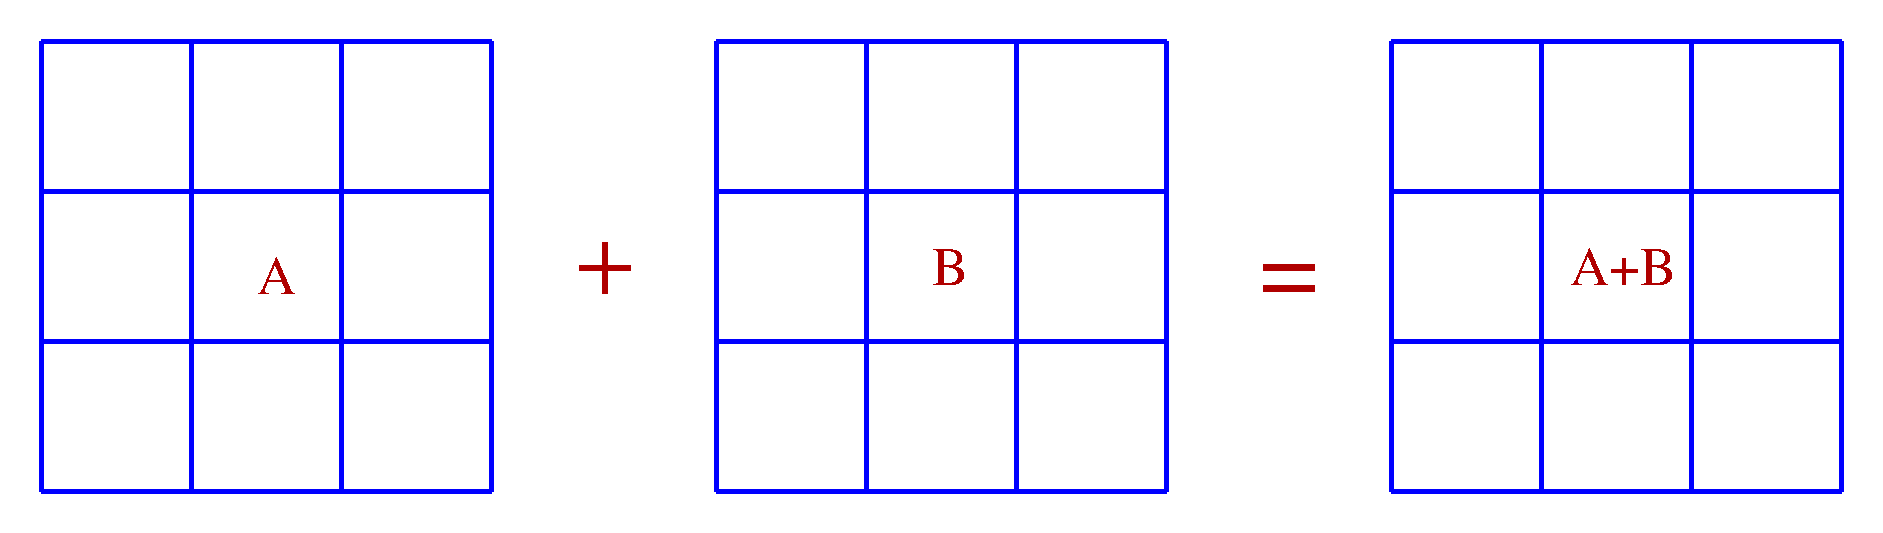
\epsfig{file=magicsqs.eps, height=3cm}\\[.3cm]
\refstepcounter{figure} \label{Cone3x3} Figure \thefigure: Magic
squares form a cone
\end{center}
\vspace*{-0.3cm}
\end{figure}

Clearly, addition of two magic squares gives another magic square,
as well as does multiplication of a magic square by a non-negative
number. Therefore, we may talk about the cone of magic $3\times 3$
squares.

This cone is a pointed rational cone described by 
$A_{3\times 3}z=0$, $z\geq 0$, where
\[
A_{3\times 3}=
\left(
\begin{array}{rrrrrrrrr}
1 & 1 & 1 & -1 & -1 & -1 &  0 &  0 &  0\\
1 & 1 & 1 &  0 &  0 &  0 & -1 & -1 & -1\\
0 & 1 & 1 & -1 &  0 &  0 & -1 &  0 &  0\\
1 & 0 & 1 &  0 & -1 &  0 &  0 & -1 &  0\\
1 & 1 & 0 &  0 &  0 & -1 &  0 &  0 & -1\\
0 & 1 & 1 &  0 & -1 &  0 &  0 &  0 & -1\\
1 & 1 & 0 &  0 & -1 &  0 & -1 &  0 &  0\\
\end{array}
\right).
\]
The equations $A_{3\times 3}z=0$ encode the conditions that all
rows, columns and main diagonals have the same sum as the first
row.

Our main interest, of course, is in integer magic squares, and from
this point on, we will only consider integer magic squares.
In particular, we would like to know a Hilbert basis of the cone
$\{z:A_{3\times 3}z=0,z\geq 0\}$, which generates all other magic
squares as \important{nonnegative integer} linear combinations.

We create an input file \File{A3x3} for \FourTiTwo{} which looks as
follows:
\begin{myverbatim}
7 9
1 1 1 -1 -1 -1  0  0  0
1 1 1  0  0  0 -1 -1 -1
0 1 1 -1  0  0 -1  0  0
1 0 1  0 -1  0  0 -1  0
1 1 0  0  0 -1  0  0 -1
0 1 1  0 -1  0  0  0 -1
1 1 0  0 -1  0 -1  0  0
\end{myverbatim}
and invoke \FourTiTwo{} via
\begin{myverbatim}
./hilbert A3x3
\end{myverbatim}
This call will create an output file \File{A3x3.hil} that looks like:
\begin{myverbatim}
5 9
1 2 0 0 1 2 2 0 1
0 2 1 2 1 0 1 0 2
1 1 1 1 1 1 1 1 1
2 0 1 0 1 2 1 2 0
1 0 2 2 1 0 0 2 1
\end{myverbatim}
Thus, there are $5$ minimal magic $3\times 3$ squares that
cannot be written as a sum of two other (non-zero) magic $3\times 3$
squares (see Figure \ref{hilbert3x3}).

\begin{figure}[tbh]
\begin{center}
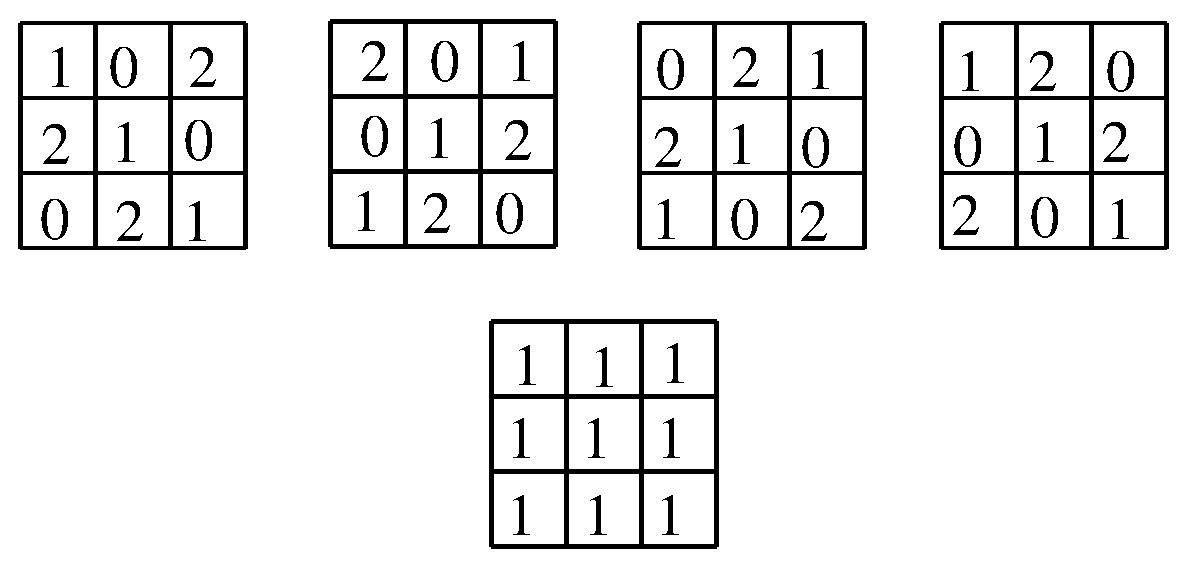
\epsfig{file=3by3magic.eps, height=5cm}\\[.3cm]
\refstepcounter{figure} \label{hilbert3x3} Figure \thefigure:
Minimal $3\times 3$ integer magic squares
\end{center}
\vspace*{-0.3cm}
\end{figure}

Moreover, any other magic $3\times 3$ square is a non-negative integer
linear combination of these $5$ squares, by the Hilbert basis property.

In order to \emph{convince} \FourTiTwo{} to create a file
\File{A3x3.hil.3way} that contains the $5$ magic squares as neat $3\times
3$ arrays, simply type
\begin{myverbatim}
./output --3way 3 3 1 A3x3.hil
\end{myverbatim}

\begin{Remark}
  \FourTiTwo{} is able to compute all minimal magic $6\times 6$
  squares, a set of more than $500,000$ elements, within $10$ days. 
  (This computation did not exploit the symmetry in the problem.)
\end{Remark}










\subsection{The 4 Coins Problem}
The following neat example is based on the one presented in
\cite{Sturmfels:03}. Let us assume that we want to give change worth
99 cents using only pennies ($1$ct), nickels ($5$ct), dimes ($10$ct),
and quarters ($25$ct). Clearly, 
\[
4\cdot 1+4\cdot 5+0\cdot 10+3\cdot 25=99
\]
would be one way to do it. Is this there another choice of $11$ coins
that sums up to $99$ct but uses fewer nickels and quarters (in total)?
In other words, we would like to solve
\[
\min\{x_2+x_4:x_1+x_2+x_3+x_4=11,x_1+5x_2+10x_3+25x_4=99,
x_1,x_2,x_3,x_4\in\Z_+\}
\]
Let us set up the problem in \FourTiTwo{}. Write the matrix into
 \File{4coins}.
\begin{myverbatim}
2 4
1 1  1  1
1 5 10 25
\end{myverbatim}
Write the cost vector into \File{4coins.cost}.
\begin{myverbatim}
1 4
0 1 0 1
\end{myverbatim}
Finally, write the known feasible solution into \File{4coins.feas}.
\begin{myverbatim}
1 4
4 4 0 3
\end{myverbatim}
Solve the problem.
\begin{myverbatim}
./minimize 4coins
\end{myverbatim}
From the output on the screen, which is also written to
\File{4coins.min}, we conclude that
\[
4\cdot 1+1\cdot 5+4\cdot 10+2\cdot 25=99
\]
is an optimal choice, using only $3$ instead of $7$ nickels and
quarters. 

\begin{Remark}
  You could also specify a list of feasible solutions in
  \File{4coins.feas}. The call
\begin{myverbatim}
./minimize 4coins
\end{myverbatim}
creates a file \File{4coins.min} containing minima to the
corresponding integer programs. (If $z_0$ is a feasible solution, the
corresponding integer program is defined by putting the right-hand
side to $Az_0$.)

You need to specify a feasible solution at the moment. It is planned
that in a future version of \FourTiTwo{} you will only need to specify
the right-hand side in \File{4coins.rhs}.
\end{Remark}









\subsection{Markov Bases in Statistics}
Let us consider the following $4\times 4$ table of non-negative
integer numbers together with all row and column sums.
\[
\begin{array}{cc}
\left(
\begin{array}{rrrr}
11 & 23 & 34 &  3\\
 4 & 15 & 12 & 11\\
17 &  2 &  3 & 25\\
16 & 12 & 22 &  7\\
\end{array}
\right)
& 
\begin{array}{r}
71\\
42\\
47\\
57\\
\end{array}\\
\begin{array}{rrrr}
48 & 52 & 71 & 46\\
\end{array} & \\
\end{array}
\]
In statistics, one often wants to sample among arrays that have fixed
counts, such as fixed row and column sums. In order to sample, one
needs a set of moves that do not change the counts when added to the
current table. Clearly, these moves must have counts $0$ and thus
quite naturally lead us a toric ideal. 

It turns out that for any set of fixed counts, a Markov
basis, that is a minimal generating set of the toric ideal, connects
all non-negative tables with these counts. That is, for any two non-negative
tables $T_1$ and $T_2$ with these counts, there is a sequence of non-negative
tables $T_1=S_0,\ldots, S_N=T_2$ with the same counts as $T_1$ and
$T_2$ and such that $S_i-S_{i-1}$ is in the Markov basis for
$i=1,\ldots, N$.

For two-way tables the situation is still very simple as our
computations with $4\times 4$ tables will now demonstrate.
Write the matrix that defines our toric ideal in \File{4x4}:
\begin{myverbatim}
8 16
1 1 1 1 0 0 0 0 0 0 0 0 0 0 0 0
0 0 0 0 1 1 1 1 0 0 0 0 0 0 0 0
0 0 0 0 0 0 0 0 1 1 1 1 0 0 0 0
0 0 0 0 0 0 0 0 0 0 0 0 1 1 1 1
1 0 0 0 1 0 0 0 1 0 0 0 1 0 0 0
0 1 0 0 0 1 0 0 0 1 0 0 0 1 0 0
0 0 1 0 0 0 1 0 0 0 1 0 0 0 1 0
0 0 0 1 0 0 0 1 0 0 0 1 0 0 0 1
\end{myverbatim}
Let us compute the Markov basis via the call
\begin{myverbatim}
./markov 4x4
\end{myverbatim}
We see that the Markov basis has $36$ elements. Let us arrange them
into $4\times 4$ arrays with the call
\begin{myverbatim}
./output --3way 4 4 1 4x4.mar
\end{myverbatim}
and have a look into the file \File{4x4.mar.3way}. We are led to the
conclusion that, up to symmetry, the Markov basis consists of the
single move
\[
\begin{array}{rrrr}
 1 & -1 &  0 &  0\\
-1 &  1 &  0 &  0\\
 0 &  0 &  0 &  0\\
 0 &  0 &  0 &  0\\
\end{array}.
\]
In fact, it can be proved that this remains true for any choice of
two-way tables.

Let us now use \FourTiTwo{} to find this one representative under
symmetry for us. (Clearly, we do not want to search for orbit
representatives in bigger Markov bases or other sets by hand.) First,
of course, we have to specify generators for the symmetries. For this,
note that swapping two rows or two columns does not change the
kernel. Write the generators into the file \File{4x4.mar.sym}:
\begin{myverbatim}
4 16
2 3 4 1 6  7  8  5 10 11 12  9 14 15 16 13
2 1 3 4 6  5  7  8 10  9 11 12 14 13 15 16
5 6 7 8 9 10 11 12 13 14 15 16  1  2  3  4
5 6 7 8 1  2  3  4  9 10 11 12 13 14 15 16
\end{myverbatim}
and call
\begin{myverbatim}
./output --sym 4x4.mar
\end{myverbatim}
which creates the file \File{4x4.mar.rep}:
\begin{myverbatim}
1 16
1 0 0 -1 0 0 0 0 0 0 0 0 -1 0 0 1 
\end{myverbatim}
Another call
\begin{myverbatim}
./output --3way 4 4 1 4x4.mar.rep
\end{myverbatim}
finally supports our original claim (see \File{4x4.mar.rep.3way}):
\begin{myverbatim}
4 4 1 1
===============
1 0 0 -1 0 0 0 0 0 0 0 0 -1 0 0 1 
===============
 1  0  0 -1 
 0  0  0  0 
 0  0  0  0 
-1  0  0  1 
===============
\end{myverbatim}

\begin{Remark}
  Nicholas Eriksson, UC Berkeley, just recently reported to
  have used \FourTiTwo{} successfully to compute toric Gr\"obner bases
  and Markov bases of ideals in $2,048$ variables!
\end{Remark}













\begin{comment}
%%%%%%%%%%%%%%%%%%%%%%%%%%%%%%%%%%%%%%%%%%%%%%%%%%%%%%%%%%%%%%%%%%%
%%%%%%%%%%%%%%%%%%%%%%%%%%%%%%%%%%%%%%%%%%%%%%%%%%%%%%%%%%%%%%%%%%%
%\newpage

\section{Release Information}

\subsection{Platform and Memory Requirements}

The binaries for \FourTiTwo{} v1.1 are available for (Sun machines and
for) platforms that run Linux. They were compiled using \Command{gcc}
version 2.96. This or a higher version of \Command{gcc} is needed to
run \FourTiTwo{}. The memory requirements are essentially problem
dependent and they can easily exceed 1GB of RAM for tough problems.





\subsection{File Descriptions} 
The Linux release of \FourTiTwo{}, version 1.1, consists of a single
archive file, 
\[
\important{4ti2\_linux\_v1.1.tar.gz},
\]
that contains the following files:
 
\begin{tabular}{|l|l|}
\hline
Name & Description\\
\hline 
%\hline
%& \\
graver & Main program executables\\
groebner & \\
hilbert & \\
markov & \\
minimize & \\
%& \\
\hline
%& \\
circuits & Additional useful executables\\
cleanup & \\
genModel & \\
genSymm & \\
output & \\
poincare & ($\gets$ only available for Linux)\\ 
%& \\
\hline
%& \\
EXAMPLES/ & Subdirectory containing sample input files\\
%& \\
\hline
%& \\
manual\_v1.1.ps & User's guide in Postscript and PDF formats\\
manual\_v1.1.pdf & \\
%& \\
\hline 
\end{tabular}


\subsection{How to Cite \FourTiTwo{}}

Although \FourTiTwo{} is free software for non-commercial use, your
acknowledgment is required. If \FourTiTwo{} is useful in your research
or applications please acknowledge it by referencing it as 
\begin{myverbatim}
@Misc{4ti2,
  author = {4ti2 team},
  title  = {4ti2--A software package for algebraic, geometric
            and combinatorial problems on linear spaces},
  howpublished = {Available at www.4ti2.de}
}
\end{myverbatim}




\subsection{The \FourTiTwo{} Team}
\begin{itemize}
\item Ralf Hemmecke (RISC, University of Linz, Austria)
\item Raymond Hemmecke (University of Magdeburg, Germany)
\item Matthias K\"oppe (University of Magdeburg, Germany)
\item Peter Malkin (CORE, Universit\'e catholique de Louvain, Belgium)
\item Matthias Walter (University of Magdeburg, Germany)
\end{itemize}



\subsection{Acknowledgments}

We are truly grateful to several people for many suggestions and
interesting conversations that led to an improvement of our
software. In the dearest hope that we do not forget someone in the
following collection of names, our thanks goes to (in alphabetical
order): Maya Ahmed, Jes\'us De Loera, Serkan Hosten, Diana Maclagan,
Kristen Nairn, R\"udiger Schultz, Bernd Sturmfels, Seth Sullivant,
Rekha Thomas, Ruriko Yoshida. 


\end{comment}



\begin{thebibliography}{99}
\bibitem{Sturmfels:03}
Sturmfels, B.: Algebraic recipes for integer programming. 
eprint arXiv:math.OC/0310194, 2003.
\end{thebibliography}	


\end{document}
